\documentclass[11pt]{article}
\usepackage[left=20mm, right=20mm,top=20mm, bottom= 20mm]{geometry}
\usepackage{verbatim, graphicx, tcolorbox}
\usepackage{multirow, makecell, url}
\usepackage{subcaption}

\title{Canonical Correlation Analysis Report for "Life Expectancy" Dataset}
\author{S/18/827 - J Kumudumali Sandaleka}
\date{\today}


\begin{document}
	
	\maketitle
	\setlength{\parindent}{0pt}
	\setlength{\parskip}{6pt}
	
	\section{Introduction}
	Canonical Correlation Analysis (CCA) is a multivariate statistical technique that identifies and measures the associations between two sets of variables. Unlike simple correlation, which assesses the relationship between two variables, CCA simultaneously examines the relationships between two multivariate sets of variables. This analysis is particularly useful in understanding complex phenomena where multiple factors from two distinct domains interact.
	
	In this project, my primary question driving is: "How are various health factors associated with immunization and economic factors in determining life expectancy?" The purpose of this study is to identify the underlying correlations that might inform public health policy and resource allocation. This analysis is crucial as it provides insights into how interconnected health and economic factors impact life expectancy, guiding health interventions and policy decisions.
	
		\subsection{Dataset Description}
		The dataset for this analysis, sourced from the WHO's Global Health Observatory and supplemented with economic data from the United Nations, encompasses life expectancy and critical health factors for 193 countries from 2000 to 2015. This period reflects significant health sector advancements, especially in developing nations.
		
		The followings are the variables,
		
		\begin{itemize}
			\item Country : Country
			\item Year : Year
			\item Life expectancy : Life Expectancy in age		
			\item Adult Mortality : Adult Mortality Rates of both sexes (probability of dying between 15 and 60 years per 1000 population)		
			\item infant deaths : Number of Infant Deaths per 1000 population		
			\item Alcohol : Alcohol, recorded per capita (15+) consumption (in litres of pure alcohol)		
			\item percentage expenditure : Expenditure on health as a percentage of Gross Domestic Product per capita(\%)		
			\item Hepatitis B : Hepatitis B (HepB) immunization coverage among 1-year-olds (\%)		
			\item Measles : Measles - number of reported cases per 1000 population		
			\item BMI : Average Body Mass Index of entire population	
			\item Polio : Polio (Pol3) immunization coverage among 1-year-olds (\%)		
			\item Total expenditure : General government expenditure on health as a percentage of total government expenditure (\%)		
			\item Diphtheria : Diphtheria tetanus toxoid and pertussis (DTP3) immunization coverage among 1-year-olds (\%)		
			\item HIV/AIDS : Deaths per 1 000 live births HIV/AIDS (0-4 years)				
			\item Schooling : Number of years of Schooling(years)
		\end{itemize}
		
	
	\section{Methodology}
	The methodology section encompasses rigorous data preprocessing, canonical correlation analysis, testing for significance, ensuring a comprehensive understanding of latent factors and their relationships within the "Life Expectancy" dataset.
	
		\subsection{Data Preprocessing}
		
		Before conducting canonical correlation analysis, the dataset was thoroughly preprocessed to ensure its integrity and suitability. This required addressing duplicate entries and missing values in addition to standardizing the data to reduce inconsistencies caused by disparate units of measurement. In this stage, it is observed that there are no outliers in this dataset. 
		
			\subsection{Statistical Methods: Canonical Correlation Analysis}
			
			Canonical Correlation Analysis (CCA) is a statistical method used to explore the relationships between two sets of variables. Unlike simpler correlation techniques that measure the relationship between two individual variables, CCA is designed to handle the complexity of relationships among multiple variables in two datasets. This method identifies pairs of canonical variates (linear combinations of the original variables) that maximize the correlation between the two sets.\\

			\textbf{\underline{Steps in Canonical Correlation Analysis}}
		
			\subsubsection{Formulating the Data Matrices:}
			The variables are categorized into health-related factors, economic factors, and immunization rates.
			
			\textbf{Set U (Health-related factors):}
			\begin{enumerate}
				\item Life expectancy
				\item Adult Mortality
				\item Infant deaths
				\item BMI
			\end{enumerate}
			
			\textbf{Set V (Immunization and Economic factors):}
			
			\begin{enumerate}
				\item Alcohol
				\item Hepatitis B
				\item Measles
				\item Polio
				\item Diphtheria
				\item Total expenditure
				\item Percentage expenditure
				\item Schooling
			\end{enumerate}
			
			\subsubsection{Canonical correlation coefficients}
			The canonical correlation coefficients are the values that indicate how strongly the two sets of variables are related. They range from 0 to 1, where 0 means no relationship and 1 means a perfect relationship. The first canonical correlation coefficient is the highest possible value, and the subsequent ones are lower and orthogonal to the previous ones. The number of canonical correlation coefficients is equal to the smaller number of variables in either set. Also, we can use the canonical correlation coefficients to test the null hypothesis that there is no relationship between the two sets of variables, and to compare the relative importance of each pair of canonical variables.
		
			
			\subsubsection{Canonical plots}
			The canonical plots are graphical representations of the canonical correlation analysis, where you can see the relationship between the two sets of variables and the cases. The most common types of canonical plots are biplots and scatter plots. A scatter plot shows the cases on the plot, where each axis represents a canonical variable. The shape and location of the points indicate the scores and clusters of the cases on the canonical dimensions.
			
			\subsubsection{Raw canonical coefficients / Canonical weights}
			The canonical weights are the coefficients that are used to create the canonical variables from the original variables. They are similar to the regression coefficients in multiple regression, and they indicate how much each variable contributes to the formation of the canonical variable. The canonical weights can help us determine which variables are most important or influential in creating the canonical variables, and how they affect the canonical correlation.
			
			
			\subsubsection{Canonical loadings}
			Canonical loadings are the correlations between the original variables and the canonical variables, which are linear combinations that maximize the canonical correlation coefficients. They help interpret the meaning and direction of the canonical variables and their relationships. A high positive loading indicates that a variable contributes positively to the canonical correlation and is positively associated with other variables with high positive loadings on the same canonical variable.
			
			\subsubsection{Canonical cross-loadings}
			Canonical cross-loadings measure the correlations between the original variables and the canonical variables of the other set. They help assess the overlap or redundancy between the two sets of variables and their mutual influence. A high positive cross-loading indicates a strong correlation with the canonical variable of the other set, sharing common variance with variables that have high loadings on that canonical variable. Canonical cross-loadings also help compute canonical communality, which quantifies the shared variance between the two sets of variables.

	\section{Results and Discussion}
		\subsection{Testing for Significance}
		
		To test for independence between the health-related factors and the immunization and economic factors,
		
			\begin{tcolorbox}[colback=white, colframe=white]
				\begin{verbatim}
					Wilks' Lambda, using F-approximation (Rao's F):
					stat    approx df1      df2      p.value
					1 to 4:  0.2669098 81.275272  32 6038.553 0.000000e+00
					2 to 4:  0.6810853 32.056865  21 4704.002 0.000000e+00
					3 to 4:  0.9546040  6.419760  12 3278.000 2.120193e-11
					4 to 4:  0.9920124  2.641023   5 1640.000 2.188721e-02
					
					
					 Hotelling-Lawley Trace, using F-approximation:
					stat     approx df1  df2      p.value
					1 to 4:  2.00057543 102.248160  32 6542 0.000000e+00
					2 to 4:  0.44883164  34.998182  21 6550 0.000000e+00
					3 to 4:  0.04723929   6.454068  12 6558 1.500378e-11
					4 to 4:  0.00805190   2.643439   5 6566 2.151494e-02
					
					
					Pillai-Bartlett Trace, using F-approximation:
					stat    approx df1  df2      p.value
					1 to 4:  0.940334145 63.003122  32 6560 0.000000e+00
					2 to 4:  0.332223019 28.329614  21 6568 0.000000e+00
					3 to 4:  0.045697231  6.332869  12 6576 2.809553e-11
					4 to 4:  0.007987585  2.634774   5 6584 2.189202e-02
					
					
					 Roy's Largest Root, using F-approximation:
					stat   approx df1  df2 p.value
					1 to 1:  0.6081111 318.1075   8 1640       0
					
					F statistic for Roy's Greatest Root is an upper bound.
				\end{verbatim}
			\end{tcolorbox}
			
			\begin{equation}
				H_0 : \rho_i = 0\; vs\; H_1 : at\; least\; one\; \rho_i \neq 0\; for\; i = 1,2,3,4
			\end{equation}
			
			All multivariate tests, including Wilks' Lambda, Hotelling-Lawley Trace, Pillai-Bartlett Trace, and Roy's Largest Root, indicate highly significant canonical correlations with p-values well below 0.0001. These consistently low p-values confirm the statistical significance of the canonical correlations across all canonical functions.
			
			Given that canonical correlations are ordered from largest to smallest, the results suggest that the first canonical correlation ($\rho_1$) is particularly noteworthy and significantly different from zero. This indicates a strong relationship between the first pair of canonical variates from the two sets of variables (U and V).
			
			\begin{equation}
				H_0 : \rho_i = 0\; vs\; H_1 : at\; least\; one\; \rho_i \neq 0\; for\; i = 2,3,4
			\end{equation}
			
			The second canonical correlation, though smaller than the first, remains statistically significant across all multivariate tests ($p < 0.0001$). This suggests that even after accounting for the first canonical variate, there is still a meaningful relationship between the remaining variance in the U and V sets. The second canonical function explains a notable, though lesser, portion of the shared variance.
			
			\begin{equation}
				H_0 : \rho_i = 0\; vs\; H_1 : at\; least\; one\; \rho_i \neq 0\; for\; i = 3,4
			\end{equation}
			
			The third canonical correlation also shows statistical significance ($p < 0.0001$), indicating that the third pair of canonical variates still captures a significant, albeit smaller, relationship between the two sets of variables. This suggests that there is additional, but reducing, shared variance explained by the third canonical function.
			
			\begin{equation}
				H_0 : \rho_4 = 0\; vs\; H_1 : \rho_4 \neq 0
			\end{equation}
			
			The fourth canonical correlation is statistically significant ($p < 0.0001$), though it is the smallest among the four. This implies that while the fourth pair of canonical variates accounts for the least amount of shared variance, it still represents a significant, but minimal, relationship between the sets of variables. The reducing size of the canonical correlations indicates that each successive function explains less of the remaining variance.
			
			In conclusion, all multivariate tests (Wilks' Lambda, Hotelling-Lawley Trace, Pillai-Bartlett Trace, and Roy's Largest Root) indicate significant canonical correlations. The first canonical function consistently shows the strongest relationship across all tests. These results suggest that the canonical variates derived from the two sets of variables (U and V) have significant and meaningful relationships.
			
			
		\subsection{Canonical correlation}
			The squared values of the canonical variate pairs can be interpreted similarly to how $r^2$ values are interpreted in regression analysis.
			
			\begin{tcolorbox}[colback=white, colframe=white]
				\begin{verbatim}
					Canonical.Correlation      Squared.Canonical.Correlation
						
					0.77981480                  0.608111126			
					0.53528104                  0.286525788			
					0.19418972                  0.037709646			
					0.08937329                  0.007987585
				\end{verbatim}
			\end{tcolorbox}
				
				
			From the results, we observe that 60.81\% of the variation in $U_1$ is explained by the variation in $V_1$, and 28.65\% of the variation in $U_2$ is explained by $V_2$. However, only 3.77\% of the variation in $U_3$ is explained by $V_3$, and the fourth squared canonical correlation is extremely low at 0.80\%. This indicates that the first canonical correlation is very high and suggests that it is the most significant. The subsequent canonical correlations drop off sharply, highlighting that only the first canonical correlation is truly important for understanding the relationship between the health-related factors and immunization and economic factors.
				
		\subsection{Canonical correlation plot}
			The first canonical variate for health-related factors is plotted against the first canonical variate for immunization and economic factors in the scatter plot for the first canonical variate pair:
			
			\begin{figure}[h]
				\centering
				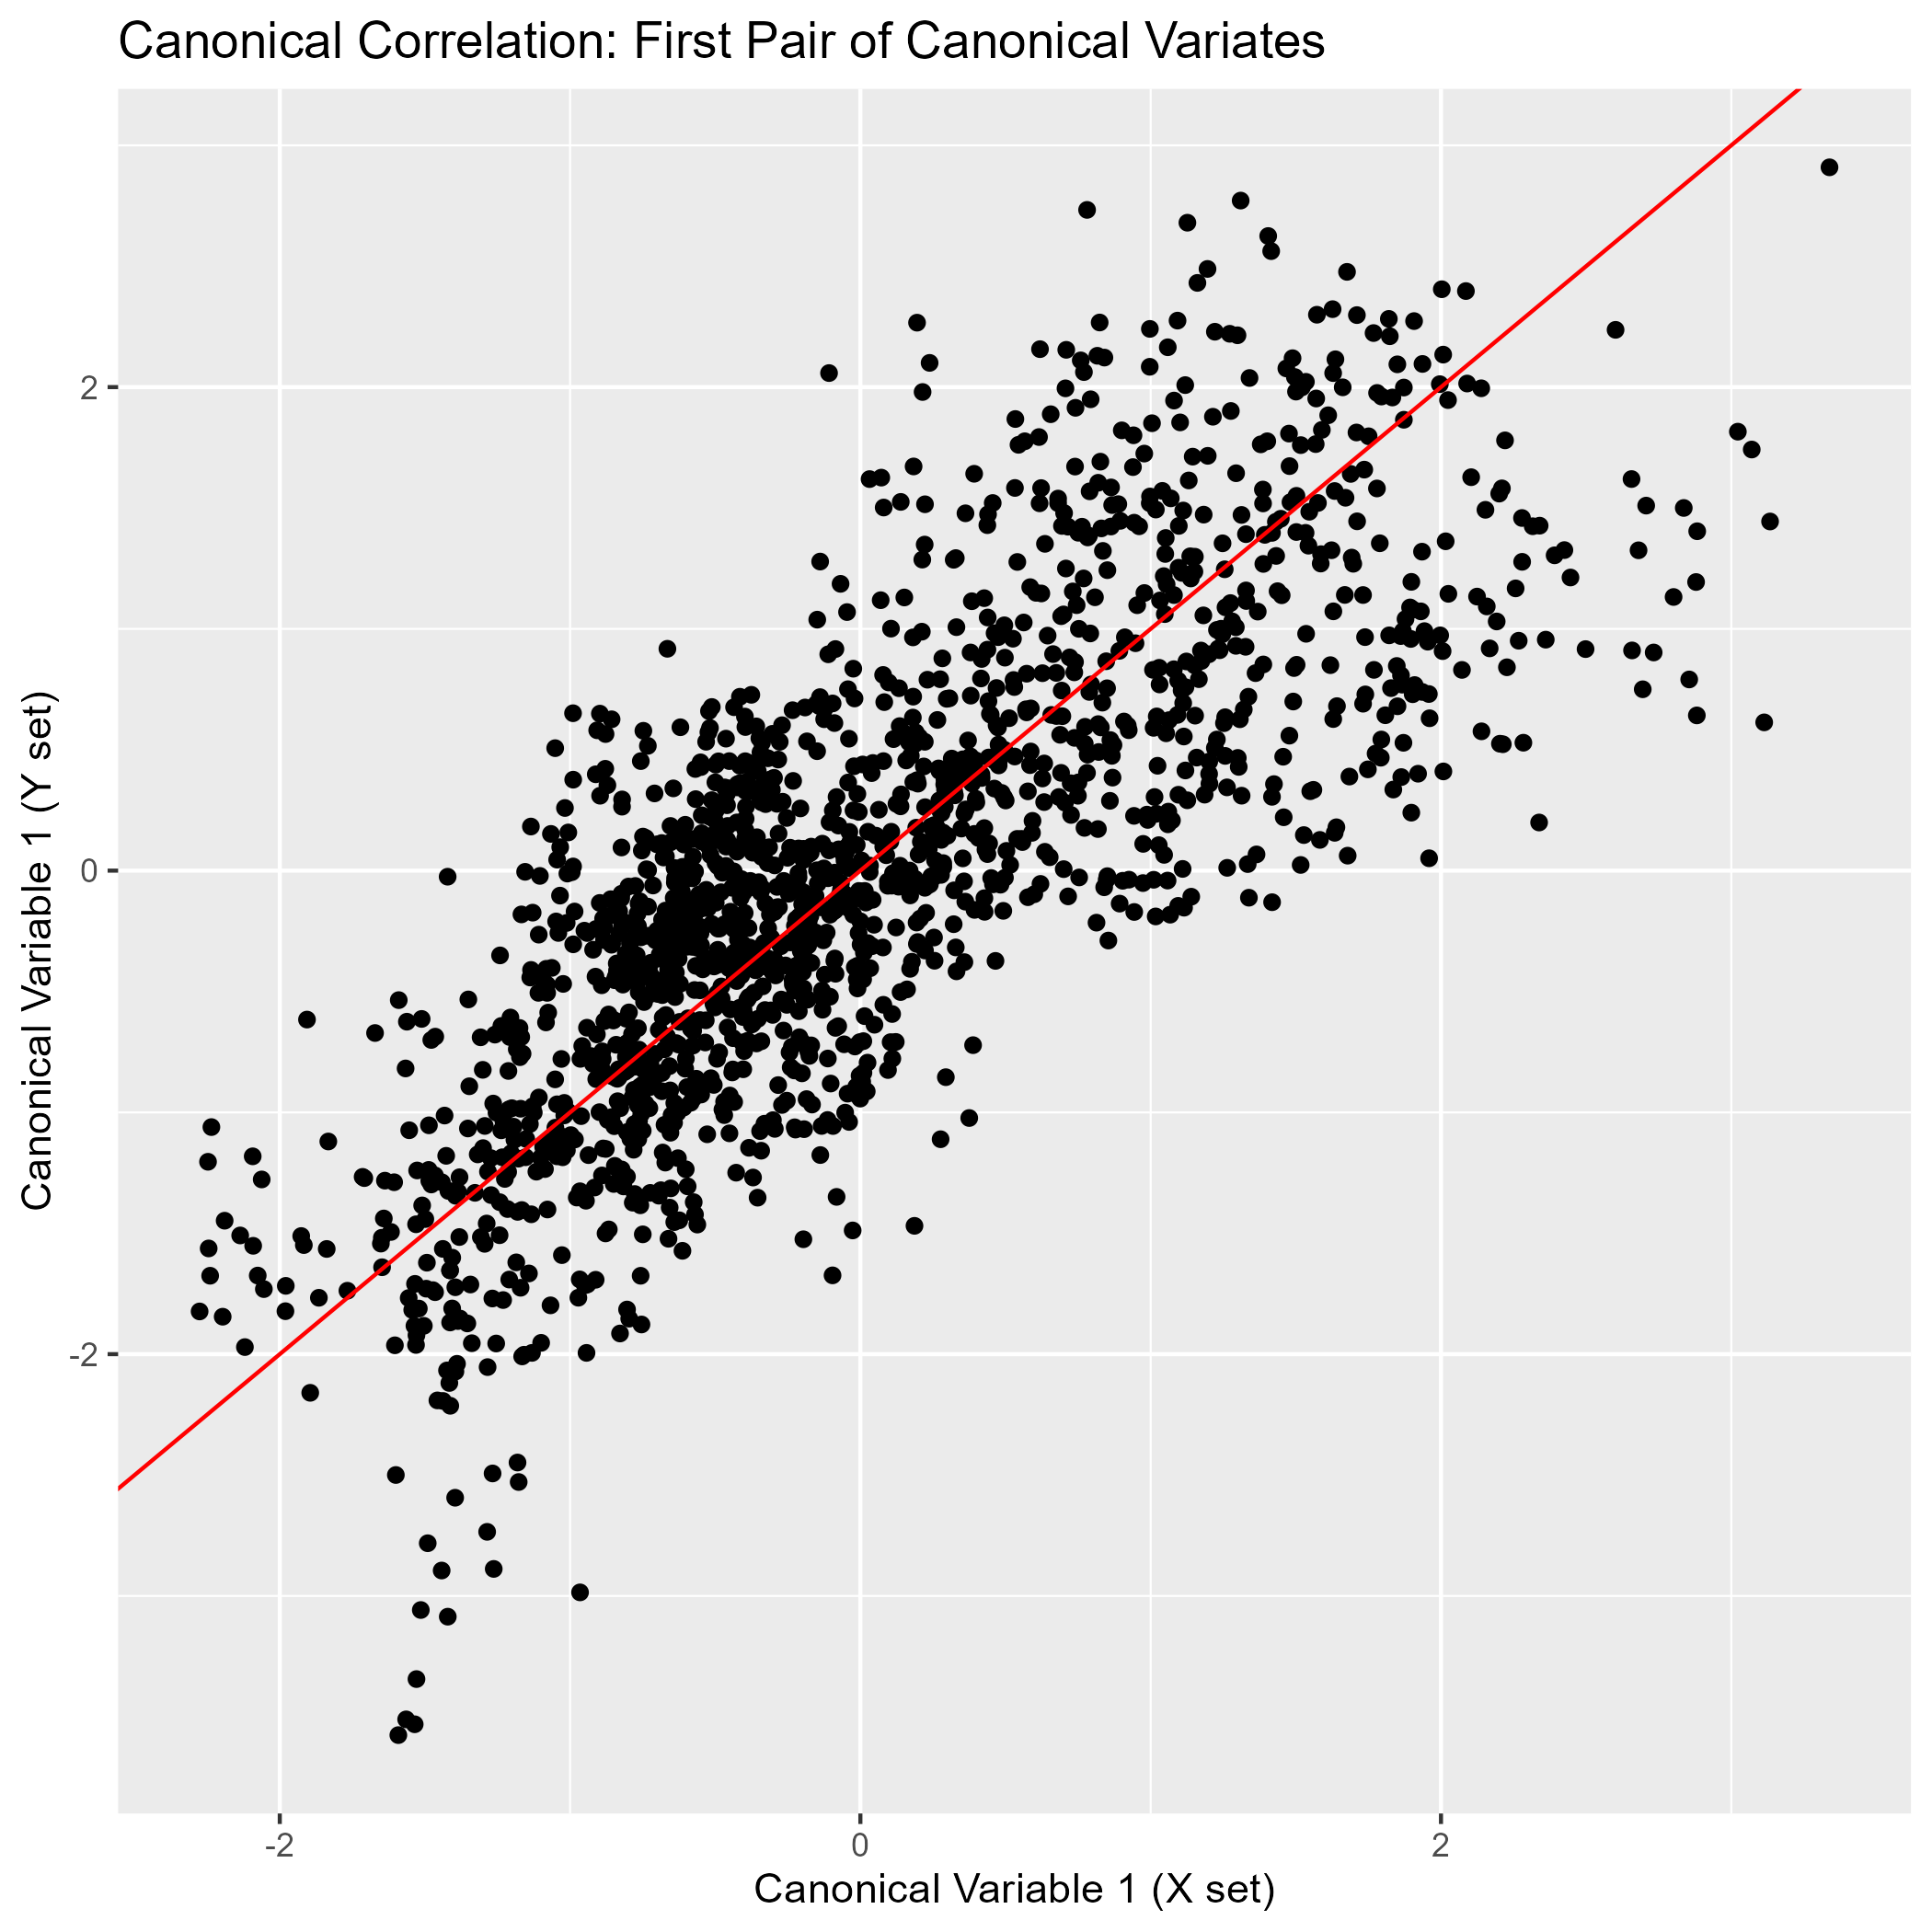
\includegraphics[width=0.5\linewidth]{../Image/first_cc_plot}
				\caption{Canonical Correlation: First Pair of Canonical Variates}
				\label{fig:firstccplot}
			\end{figure}
			The regression line shows how well the data fits. The plot is a bit more scattered, but is still a reasonably good fit.
						
		
		\subsection{Raw canonical coefficients}
		
		The raw canonical coefficients (canonical weights) are the coefficients that are used to create the canonical variables from the original variables.
		
		\begin{tcolorbox}[colback=white, colframe=white]
			\begin{verbatim}
				Set U:
				                 [,1]        
				Lifeexpectancy -0.9266450  
				AdultMortality -0.1923545  
				infantdeaths    0.1726828  
				BMI            -0.2315565 
				
			\end{verbatim}
		\end{tcolorbox}
		
		\begin{equation}
			U_1 = -0.93 X_{Life Expectancy} - 0.19 X_{Adult Mortality} + 0.17 X_{Infant Deaths} - 0.23 X_{BMI}
		\end{equation}
		
		A one-unit increase in life expectancy results in a decrease of 0.93 units in the value of the first canonical variate for the health-related set of variables, when other variables are held constant. Similarly, a one-unit increase in adult mortality and BMI leads to decreases of approximately 0.19 units and 0.23 units, respectively, in the first canonical variate. In contrast, a one-unit increase in infant deaths causes an increase of about 0.17 units in the value of the first canonical variate for the health-related set of variables, holding other variables constant.
		
		
		\begin{tcolorbox}[colback=white, colframe=white]
			\begin{verbatim}
				Set V:
				                         [,1]
				Alcohol                0.09912126 
				HepatitisB            -0.03722022 
				Measles                0.12392999  
				Polio                 -0.04655309 
				Diphtheria            -0.07482133 
				Totalexpenditure      -0.01522375
				percentageexpenditure -0.15428906
				Schooling             -0.90043023 
			\end{verbatim}
		\end{tcolorbox}
		
		\begin{equation}
			V_1 = 0.1 Y_{Alcohol} - 0.04 Y_{Hep.B} + 0.12 Y_{Measles} - 0.05 Y_{Polio} - 0.07 Y_{Diph.} - 0.02 Y_{Tot.exp} - 0.15 Y_{\% exp.} - 0.9 Y_{Sch}
		\end{equation}
		
		A one-unit increase in alcohol consumption results in a 0.10 unit increase in the value of the first canonical variate for the immunization and economic factors set, when other variables are held constant. Conversely, increases in Hepatitis B immunization, polio immunization, diphtheria immunization, total expenditure, and percentage expenditure lead to decreases of approximately 0.04 units, 0.05 units, 0.07 units, 0.02 units, and 0.15 units, respectively, in the first canonical variate. A significant impact is observed with schooling, where a one-unit increase results in a substantial decrease of approximately 0.90 units in the first canonical variate for the immunization and economic factors set, holding other variables constant.
			
		\subsection{Canonical - loadings}
			The canonical loadings are the correlations between the original variables and the canonical variables, which are the linear combinations of variables that maximize the canonical correlation coefficients.
			\begin{tcolorbox}[colback=white, colframe=white]
				\begin{verbatim}
					Set U:
					                     [,1]       
					Lifeexpectancy 		  -0.9462209 
					AdultMortality 		   0.5473673 
					infantdeaths   		   0.3754714 
					BMI               -0.7066970 
					
					Set V:
					[,1]        
					Alcohol               -0.5637043  
					HepatitisB            -0.3055000 
					Measles                0.2462906 
					Polio                 -0.4296835 
				\end{verbatim}
			\end{tcolorbox}
			
			\begin{tcolorbox}[colback=white, colframe=white]
				\begin{verbatim}
					Diphtheria            -0.4465742
					Totalexpenditure      -0.2753939
					percentageexpenditure -0.5203263
					Schooling             -0.9729704 
				\end{verbatim}
			\end{tcolorbox}
			
			The first canonical variate for the U set is strongly negatively correlated with life expectancy (-0.95) and BMI (-0.71), and positively correlated with adult and infant mortality rates. For the V set, it is negatively correlated with alcohol consumption, vaccination rates (Hepatitis B, Polio, Diphtheria), health expenditures, and years of schooling. The first canonical variate for the V set shows a strong negative correlation with years of schooling (-0.97). This suggests a significant relationship between the health metrics and the variables related to immunization and economic in these canonical variates.
			
		\subsection{Canonical cross-loadings}
			The canonical cross-loadings indicate how each original variable correlates with the canonical variate of the other set. 
			
			\begin{tcolorbox}[colback=white, colframe=white]
				\begin{verbatim}
					Set U:
					                     [,1]       
					Lifeexpectancy -0.7378771 
					AdultMortality  0.4268451
					infantdeaths    0.2927981
					BMI            -0.5510928
					
					Set V:
					            [,1]    
					Alcohol               -0.4395850  
					HepatitisB            -0.2382334 
					Measles                0.1920611
					Polio                 -0.3350736 
					Diphtheria            -0.3482452
					Totalexpenditure      -0.2147562
					percentageexpenditure -0.4057581
					Schooling             -0.7587367
				\end{verbatim}
			\end{tcolorbox}
			
		For the first set (U), Life expectancy (-0.738) and BMI (-0.551) show strong negative correlations, while Adult Mortality (0.427) and infant deaths (0.293) exhibit moderate and weak positive correlations with the canonical variate of the second set (V). For the second set (V), Schooling (-0.759) and Alcohol (-0.440) have strong and moderate negative correlations, respectively, with the first set's (U) canonical variate. Other variables such as Polio (-0.335), Diphtheria (-0.348), and percentage expenditure (-0.406) also show weak negative correlations. These cross-loadings highlight the significant inverse relationships between health metrics from the first set and immunization and economic variables from the second set.
			
			
	\section{Conclusion}
		This study applied Canonical Correlation Analysis (CCA) to explore the relationships between health-related factors and immunization and economic factors in determining life expectancy. The analysis revealed significant canonical correlations between the two sets of variables, indicating substantial relationships.
		
		Key findings include:
		
		\begin{enumerate}
			\item Significance of Canonical Correlations: All multivariate tests (Wilks' Lambda, Hotelling-Lawley Trace, Pillai-Bartlett Trace, and Roy's Largest Root) indicated highly significant canonical correlations, with p-values well below 0.0001. This underscores the robust relationships between the health-related factors and immunization and economic factors.
			
			\item Canonical Correlation Coefficients: The first canonical correlation was notably high (0.78), explaining approximately 60.81\% of the variance between the sets, indicating a strong initial relationship. Subsequent canonical correlations, while still significant, explained progressively less variance, emphasizing the dominance of the first canonical variate pair.
			
			\item Canonical Coefficients: The canonical weights and loadings provided insights into the contributions of individual variables. For example, life expectancy, BMI, and schooling had strong negative correlations with their respective canonical variates, highlighting their significant roles in the observed relationships.
			
			\item Cross-Loadings and Shared Variance: The canonical cross-loadings illustrated how variables from one set correlated with the canonical variates of the other set, further validating the interconnections between health metrics and economic and immunization factors.
		\end{enumerate}
		
		These results suggest that public health policy and resource allocation should prioritize interconnected health and economic factors to effectively enhance life expectancy. The insights gained from CCA can guide targeted interventions and strategies, ensuring a more holistic approach to improving global health outcomes.
		
		In conclusion, CCA has proven to be a powerful tool in unravelling the complex interplay between various health-related factors and economic factors, providing a comprehensive understanding that can inform and optimize public health policies.
			
	
	\section{References}
		\begin{enumerate}
			\item Abdolrasol, M. G. M., Hussain, S. M. S., Ustun, T. S., Sarker, M. R., Hannan, M. A., Mohamed, R., Ali, J. A., Mekhilef, S., \& Milad, A. (2021). Artificial Neural Networks Based Optimization Techniques: A review. Electronics, 10(21), 2689. https://doi.org/10.3390/electronics10212689 
			
			\item Canonical Correlation Analysis | R Data Analysis Examples. (n.d.). \\ https://stats.oarc.ucla.edu/r/dae/canonical-correlation-analysis/ 
			
			\item Canonical Correlation Analysis | SPSS Data Analysis Examples. (n.d.). \\
			https://stats.oarc.ucla.edu/spss/dae/canonical-correlation-analysis/ 
			
			\item Canonical Correlation Analysis | STATA Data Analysis Examples. (n.d.). \\
			https://stats.oarc.ucla.edu/stata/dae/canonical-correlation-analysis/ 
			
			\item Hair, J. F., Jr., Anderson, R. E., Tatham, R. L., Black, W. C., \& Prentice Hall, Inc. (1998). Canonical Correlation Analysis. In Canonical Correlation Analysis. https://mvstats.com/wp-content/uploads/2022/02/Canonical\_Correlation\_6e.pdf 
			
			\item Haykir, M., \& Çalışkan, O. (2021). Is There a Relationship between Empowering Chefs and the Culinary Creativity Process? Journal of Culinary Science \& Technology, 21(3), 404–429. https://doi.org/10.1080/15428052.2021.1955793 
			
			\item Lesson 13: Canonical Correlation Analysis | STAT 505. (n.d.). PennState: Statistics Online Courses. https://online.stat.psu.edu/stat505/lesson/13
		\end{enumerate}
	
	
	\section{Appendices}
	
	\begin{figure}[h]
		\centering
		
\includegraphics[width=0.7\linewidth]{../Image/1}
		\label{fig:1}
	\end{figure}
	
	\begin{figure}[h]
		\centering
		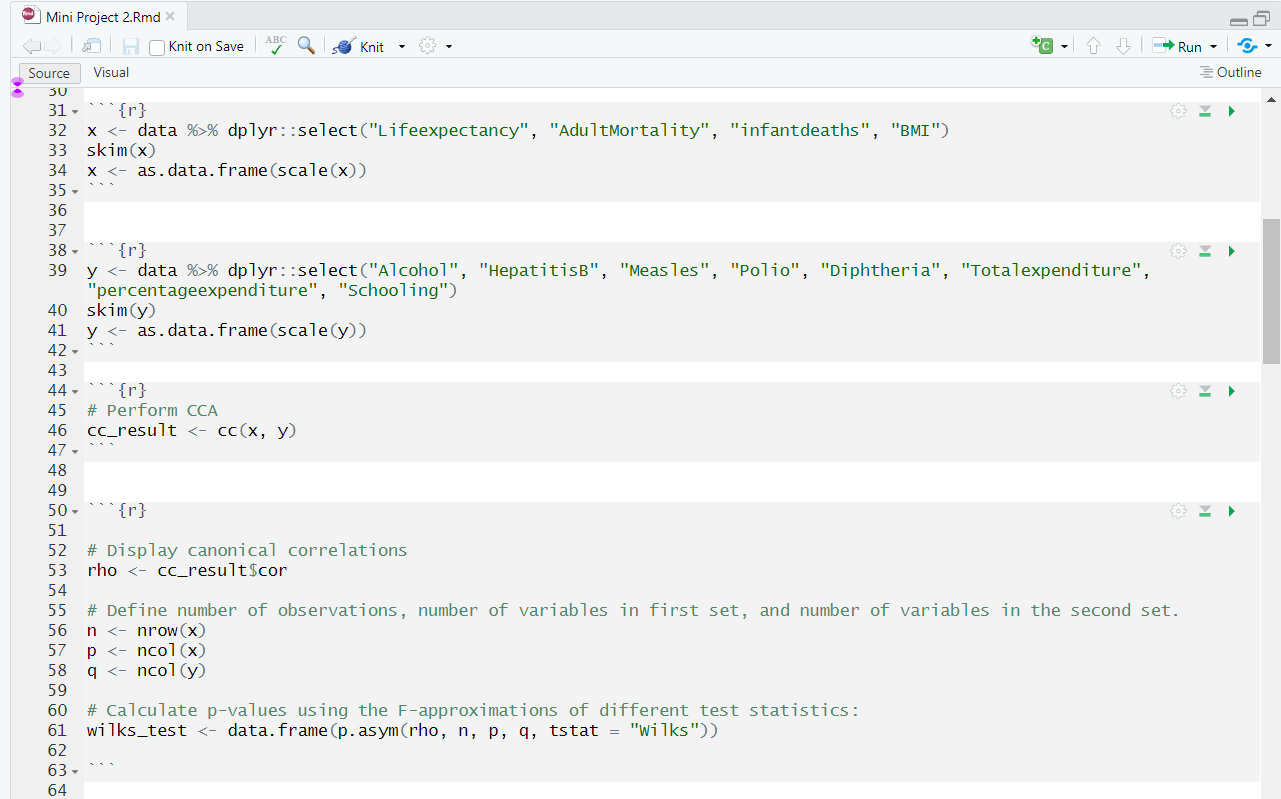
\includegraphics[width=0.7\linewidth]{../Image/2}
	\end{figure}
	
	\begin{figure}[h]
		\centering
		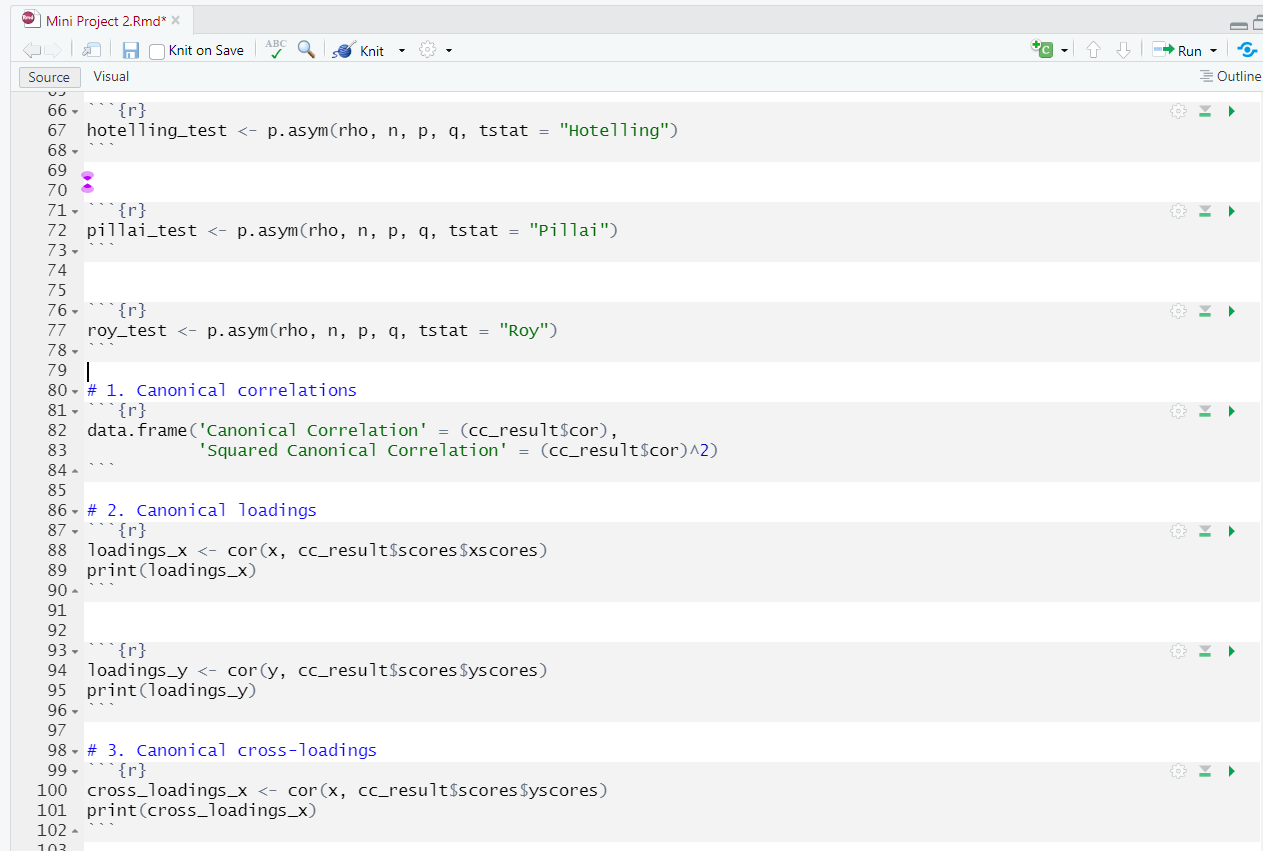
\includegraphics[width=0.7\linewidth]{../Image/3}
	\end{figure}
	
	\begin{figure}[h]
		\centering
		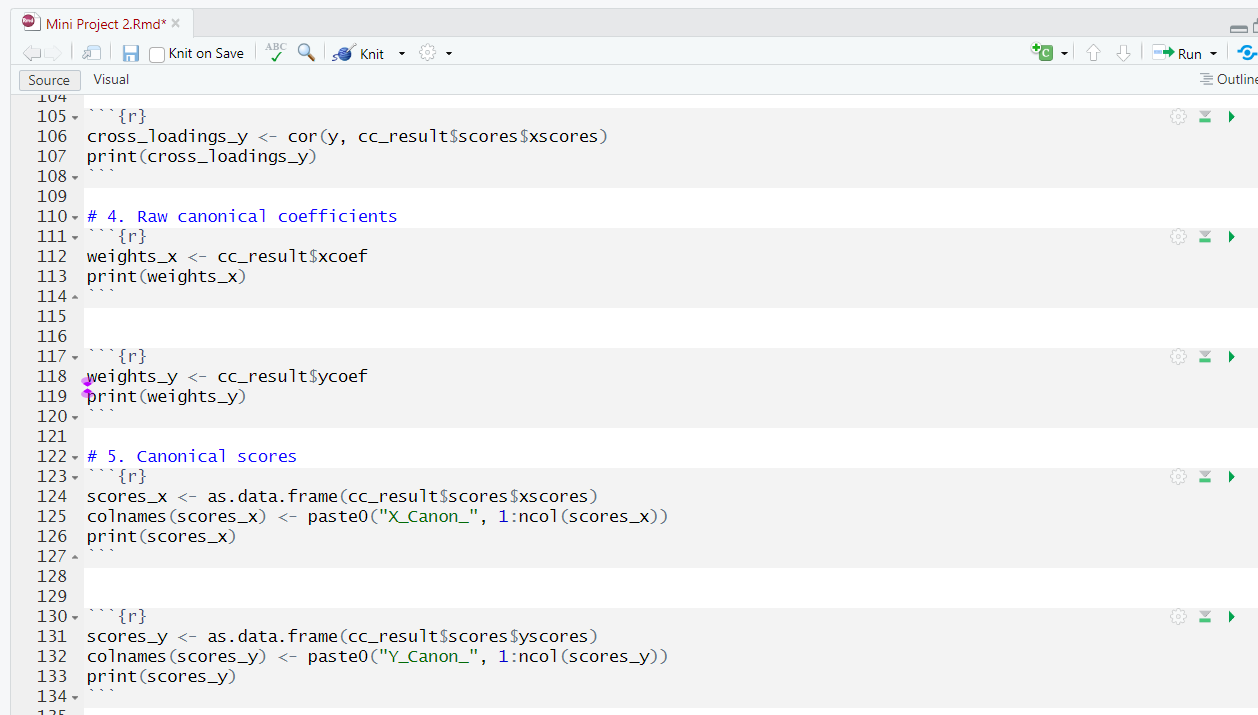
\includegraphics[width=0.7\linewidth]{../Image/4}
	\end{figure}
	
	\begin{figure}[h]
		\centering
		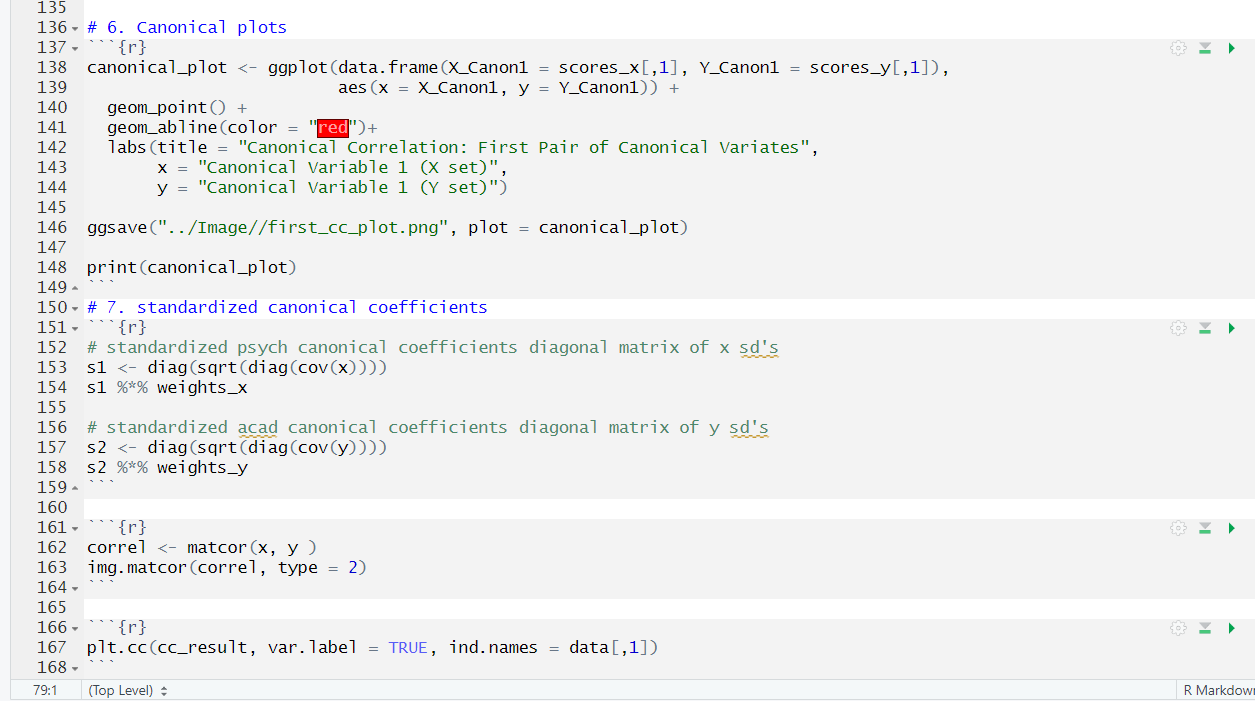
\includegraphics[width=0.7\linewidth]{../Image/5}
	\end{figure}
	
	
\end{document}
